\documentclass{article}

\usepackage[utf8]{inputenc}
\usepackage[T1]{fontenc}
\usepackage{geometry}
\usepackage{amsmath}
\usepackage{amsfonts}
\usepackage{graphicx}
\usepackage{float}
\usepackage{array}
\usepackage{tabularx}
\usepackage{booktabs}
\usepackage{algpseudocode}
\usepackage{algorithm}
\usepackage{float}
\usepackage{listings}
\usepackage{subcaption}


\usepackage{amsfonts}

\usepackage{multirow}

\title{Analyse de donnée: \
Projet \
SVM}
\author{Absobel \& SOMSON Paul}
\date{}

\begin{document}

\maketitle

\section*{Introduction}

Dans ce projet, nous avons étudié différents algorithmes de classification supervisée, et comparé leur efficacité. Comme données, nous avons utilisé des mélanomes, définis par leur compacité et leur contraste.

Dans un premier lieu, nous avons étudié une SVM linéaire, puis d'autres SVM plus efficaces.

\section{SVM linéaire}

\subsection{Version primale}

Cet algorithme se rapporte à un problème de minimisation quadratique. On cherche à minimiser la fonction suivante:

\begin{equation}
    f(w) = \frac{1}{2} \left\| w \right\|^2
\end{equation}

Ici, w est le vecteur othogonal à la droite D qui sépare les deux classes. Miniminer ce vecteur, c'est minimiser la distance entre la droite D et les points de chaque classe. C'est sur ce principe que repose cette SVM \@.
Voici le résultat sur les données d'apprentissage. Il est important de noter que les données sont linéairement séparées, sans quoi l'algorithme est très imprécis.

\begin{figure}[H]
    \centering
    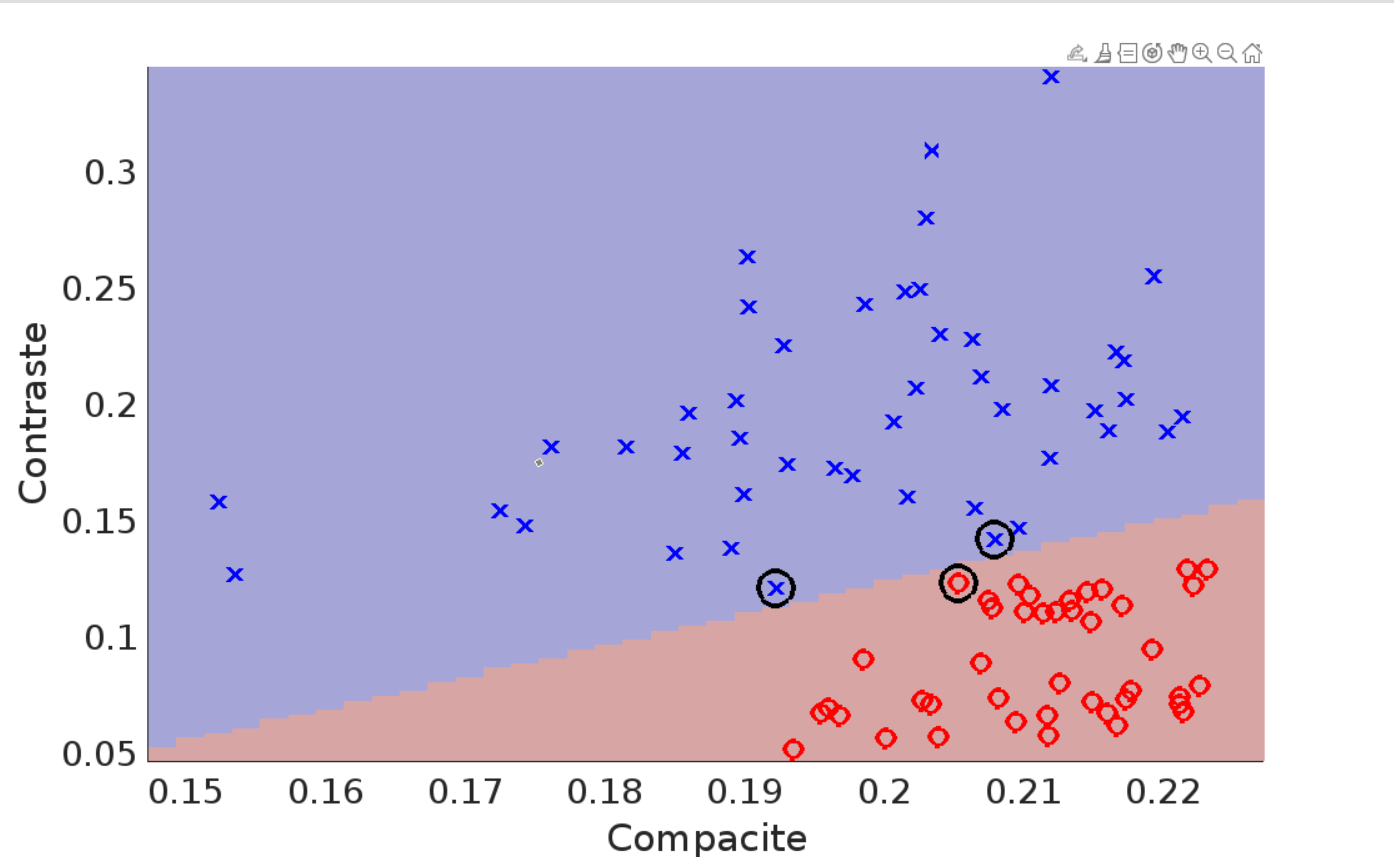
\includegraphics[width=0.5\textwidth]{images/SVM1_app.png}
    \caption{SVM linéaire primale sur les données d'apprentissage}
\end{figure}

Les données du vecteur support sont entourées sur le graphique. Cela sera le cas par la suite.

\subsection{Version duale}

Cette fois on ajoute le lagrangien, qui introduit à son tour n contraintes linéaires. Après calcul, on cherche donc à maximiser cette fonction:

\begin{equation}
    f(\alpha) = -\frac{1}{2} \alpha ^T H \alpha + f^T \alpha,   \alpha = [\alpha_1,\ldots,\alpha_n]^T
\end{equation}

avec $H_{ij} = y_i y_j x_i^T x_j$ et $f = [-1,\ldots,-1]^T$. Avec cette SVM, on obtient un résultat assez peu différent:

\begin{figure}[H]
    \centering
    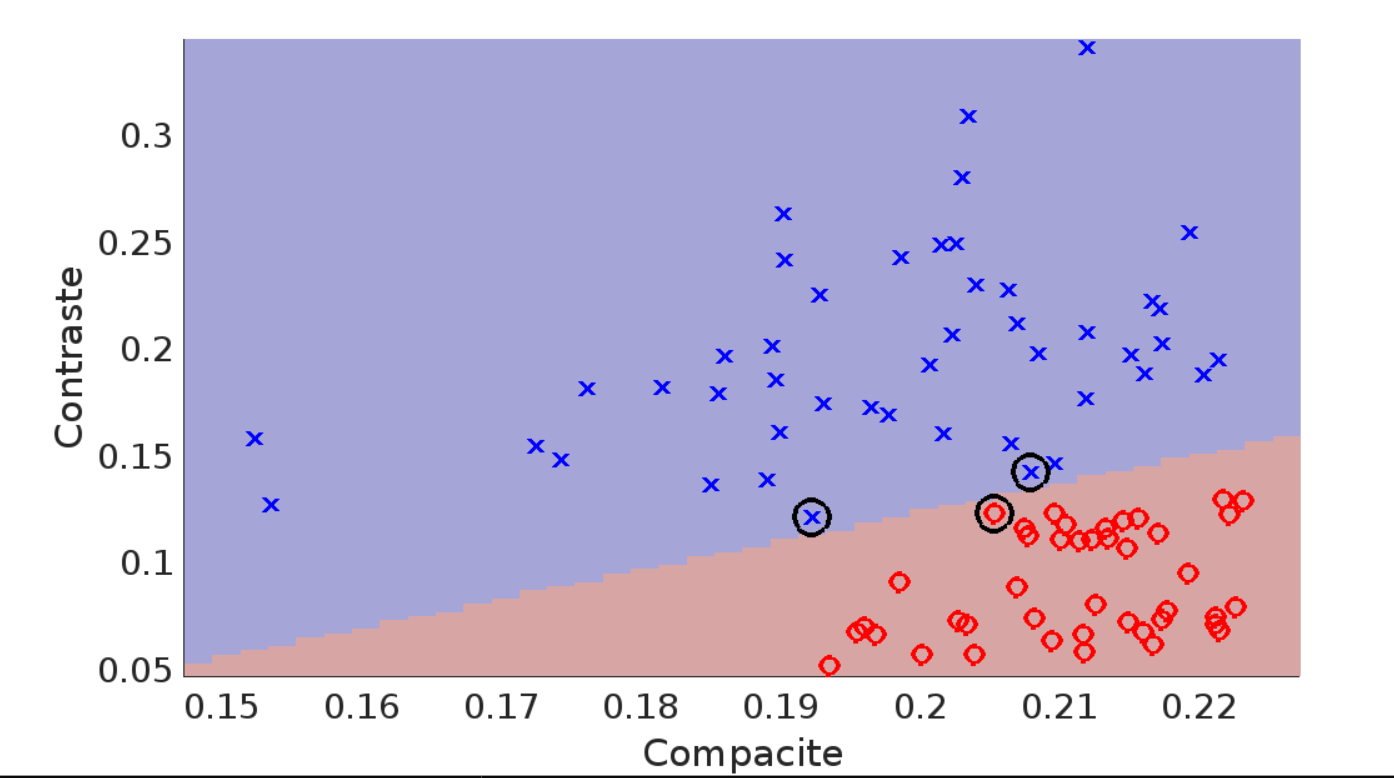
\includegraphics[width=0.5\textwidth]{images/SVM2_app.png}
    \caption{SVM linéaire duale sur les données d'apprentissage}
\end{figure}

On verra plus tard que cet algorithme permet tout de même de séparer des données non linéairement séparables avec une légère amélioration.


\section{SVM à noyau gaussien}

Les deux algorithmes précédents n'arrivent pas à séparer les données si elles sont `mélangées' (non linéairement séparables). Pour cela, on utilise une SVM à noyau gaussien.
Les données seront projetées dans un espace de dimension supérieure (ici 3), où elles pouront être séparées par un hyperplan.

\begin{figure}[H]
    \centering
    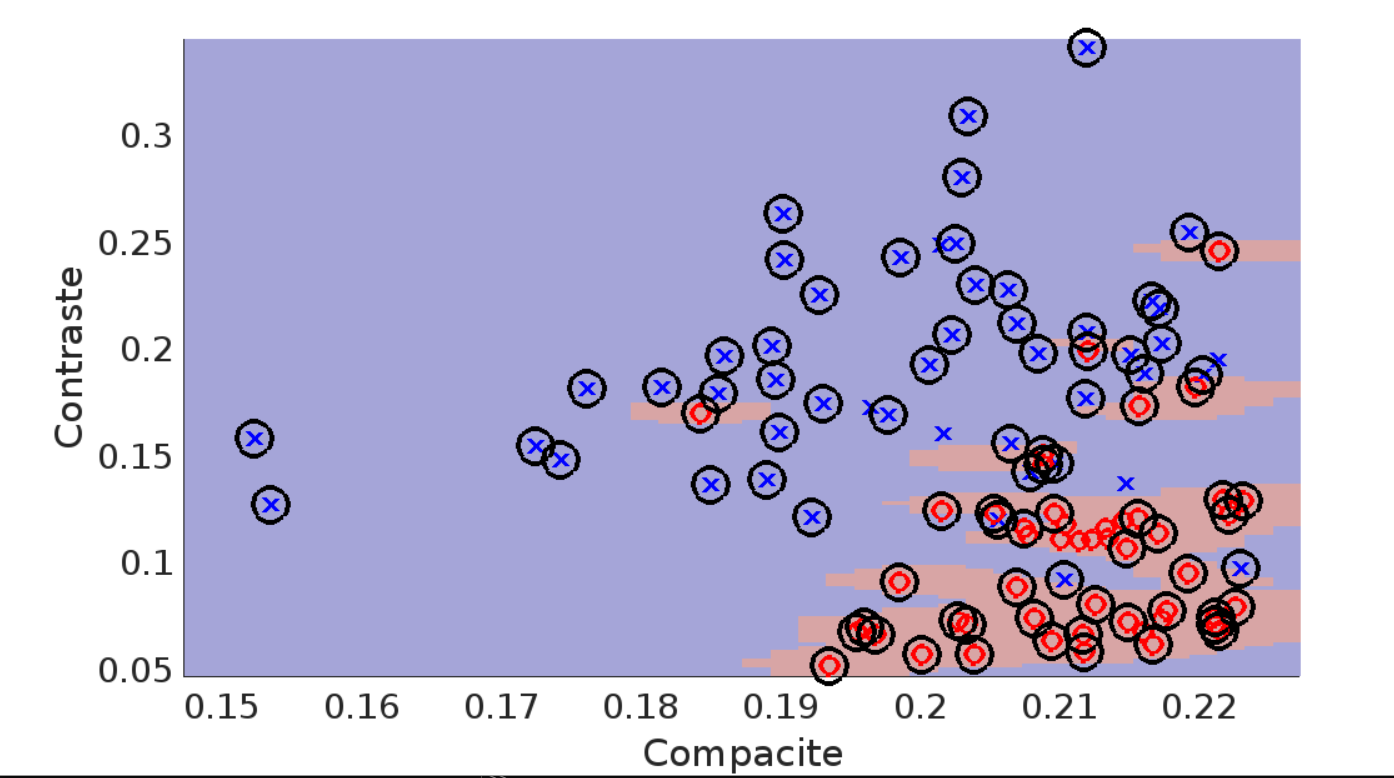
\includegraphics[width=0.3\textwidth]{images/SVM3_app.png}
    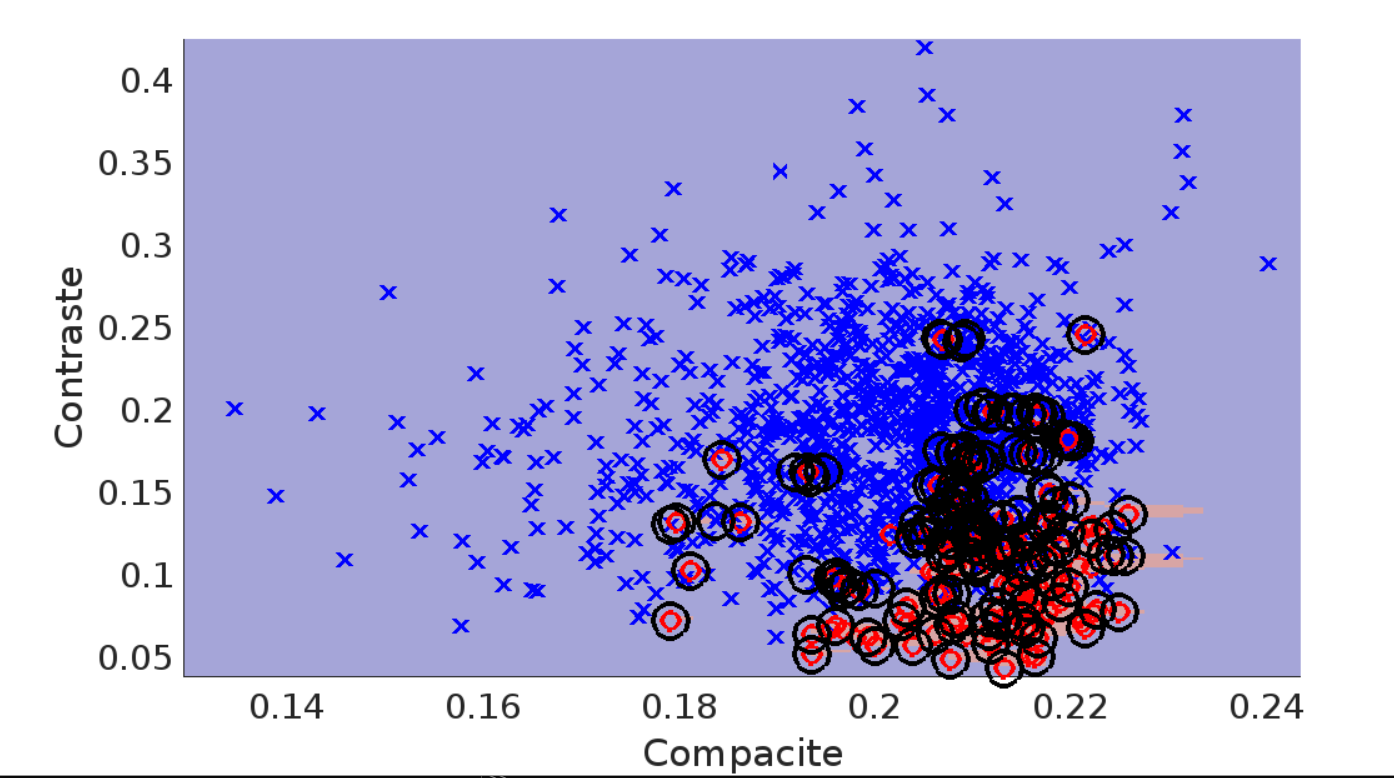
\includegraphics[width=0.3\textwidth]{images/SVM3_test.png}
    \caption{SVM à noyau gaussien sur les données d'apprentissage et de test}
\end{figure}

L'écart-type $\sigma = 0.004$ est le même pour les données d'aprentissage et de test, avec un taux de bonne classification de 90,4\% pour les données de test.
Cet algorithme est donc plus efficace que les deux précédents, mais il ne permet pas de séparer les données de manière preque parfaite. Ainsi, on va l'améliorer en assouplissant les contraintes linéaires.

\section{SVM à marge souple}

Parfois, il arrive que les contraintes linéaires soient trop rigides pour avoir une bonne classification. Par exemple dans le cas précédent, 9,6\% des données restent mal classées à cause de contraientes trop rigides.
En ajoutant des variables de ressort \lambda, il serait possible d'atteindre une meilleure précision.

\subsection{SVM linéaire à marge souple}

On reprend la SVM linéaire duale, qu'on assouplit à l'aide des variables de ressort \lambda. On cherche donc à minimiser la fonction suivante:

\begin{equation}
    f(w, \xi_1, \ldots, \xi_n) = \frac{1}{2} \left\| w \right\|^2 + \lambda \sum_{i=1}^n \xi_i
\end{equation}

avec les contraintes suivantes:

\begin{equation}
    \left\{
    \begin{array}{l}
        y_i (w^T x_i - c) - 1 \geq \xi_i \\
        \xi_i \geq 0,  \forall i \in \{1,\ldots,n\}
    \end{array}
    \right.
\end{equation}

On obtient alors le résultat suivant, avec \lambda = 10000:

\begin{figure}[H]
    \centering
    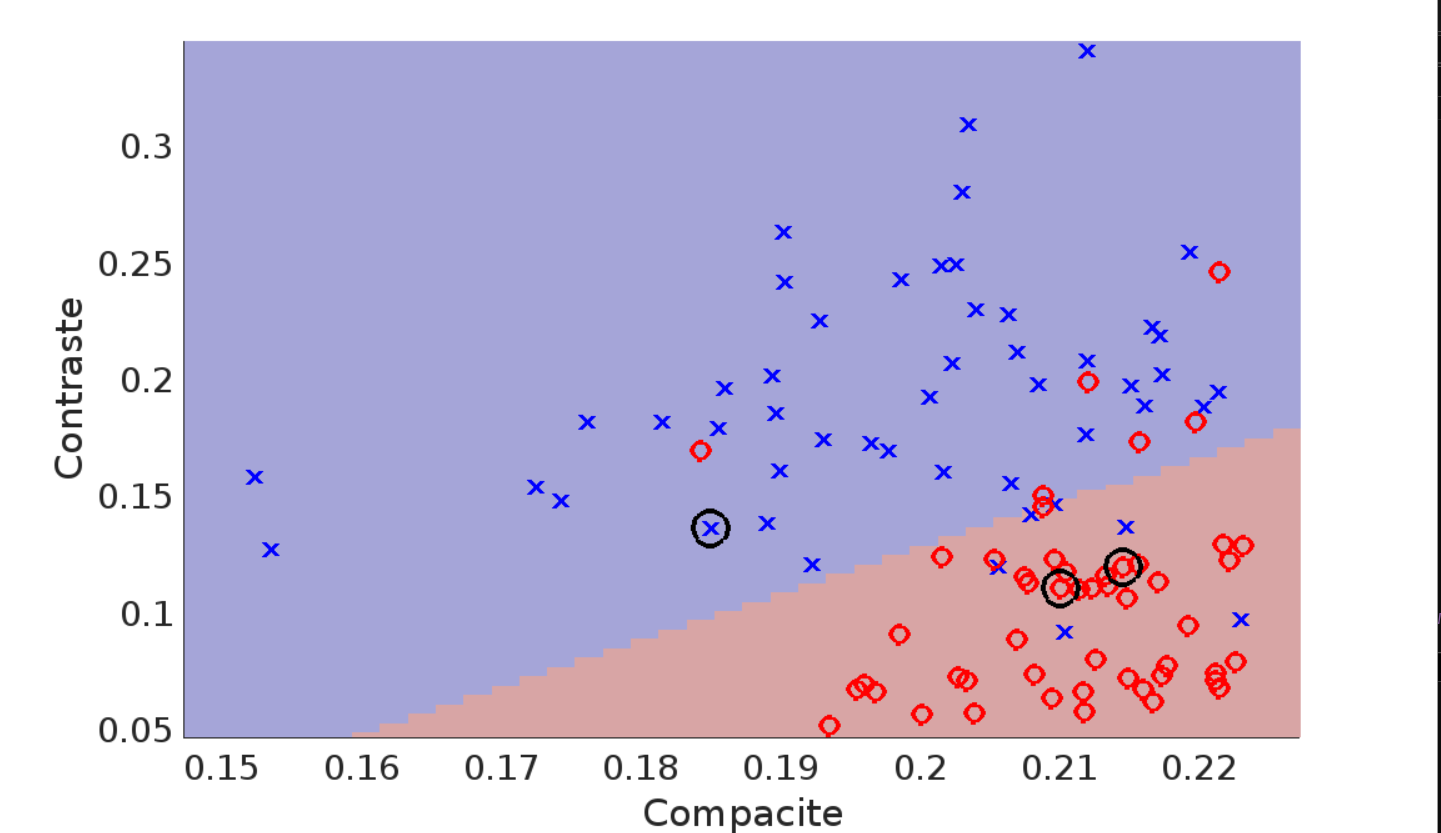
\includegraphics[width=0.5\textwidth]{images/SVM2_souple_app.png}
    \caption{SVM linéaire à marge souple sur les données d'apprentissage}
\end{figure}

Cette fois-ci les données ne sont pas linéairement séparées. La séparation n'est pas parfaite, loin de là, mais elle est bien meilleure que ce qu'aurait produit une SVM non souple. On ne peut cependant cependant pas se contenter de ces résultats.
Le défaut vient du fait qu'il est impossible de séparer le plan en deux tout en obtenant une bonne précision. pour cela, il faurait travailler dans un espace de dimension 3 ou plus.

Ainsi, on va appliquer ce principe de souplesse à la SVM avec noyau gaussien.

\subsection{SVM à noyau gaussien à marge souple}

La souplesse apportée par les variables de ressort ne change pas fondamentalement l'approche de la SVM à noyau gaussien, mais devrait fortement augmenter sa précision.

Voici les résultats obtenus avec \lambda = 1000 sur les données de test et non d'apprentissage:

\begin{figure}[H]
    \centering
    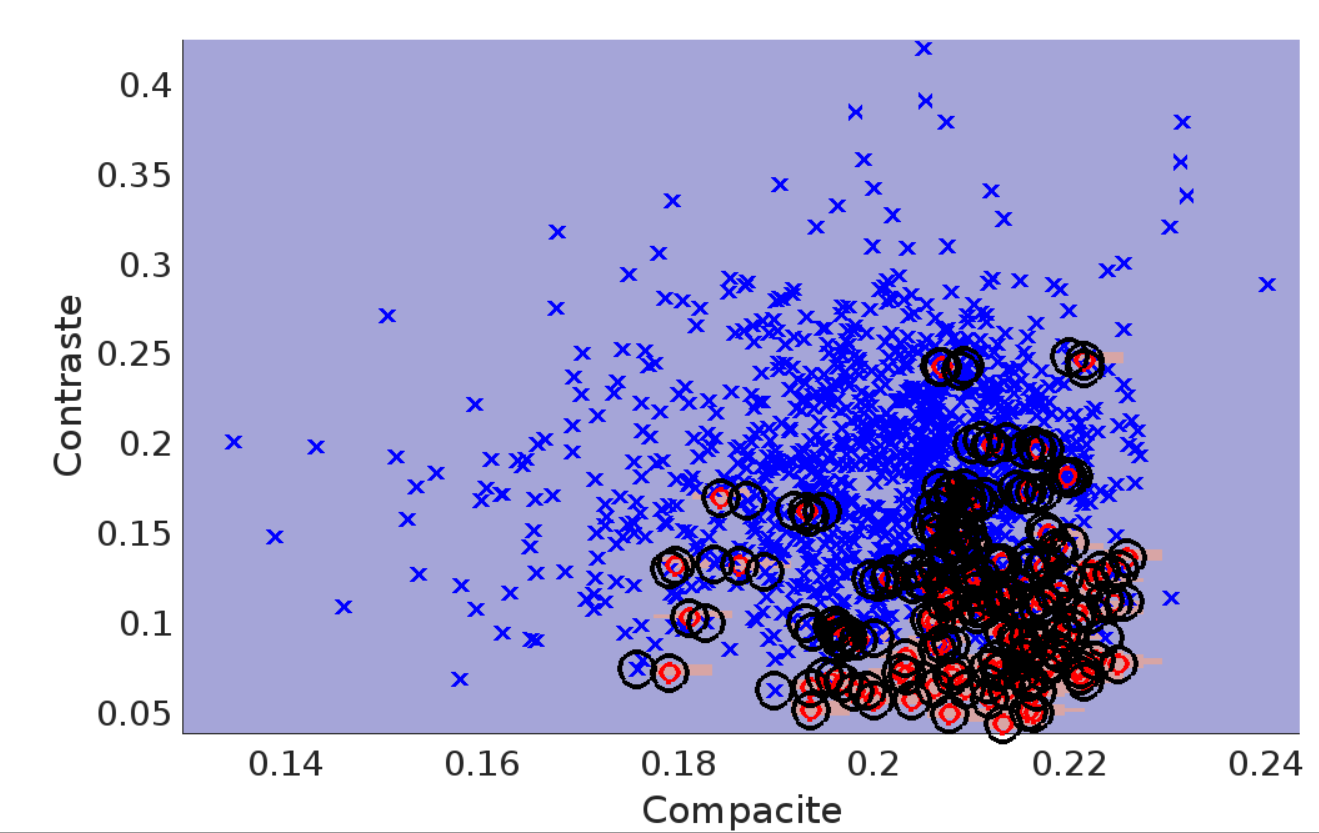
\includegraphics[width=0.5\textwidth]{images/SVM3_souple_test.png}
    \caption{SVM à noyau gaussien à marge souple sur les données d'apprentissage et de test}
\end{figure}

On obtient alors un taux de bonne classification de 99,7\% sur les données de test, ce qui est très largement suffisant. La souplesse apportée est très bénéfique, et doit certainement se généraliser bien mieux que la SVM rigide.
Cependant, le faible nombre de données de classe 2 (croix rouges) apporte un fort déséquillibre et empêche l'algorithme d'être suffisamment précis. Avec des données plus nombreuses et mieux réparties, les qualités de cette SVM devraient être beaucoup plus marquées.


\section{Conclusion}

Sans surprise, la SVM à noyau gaussien et marge souple est la plus efficace, et de loin. Pouvoir projeter les données dans un espace de dimension supérieur étant déjà redoutablement efficace pour la séparation linéaire des données, ajouter de les souplesse au modèle le rend beaucoup plus généralisable.
Les données sont malheureusement trop déséquilibrées pour pouvoir correctement juger de l'efficacité de cette SVM, mais les résultats restent très prometteurs.

De plus, le développement de ces algorithmes a été ralenti par la présence d'une ligne "NaN" à la ligne 590 des données de test, faisant échouer toute tentative de classification. Découvrir ces classificateurs resta néanmoins très passionnant.

Merci pour votre lecture.

\end{document}
